\documentclass[11pt,a4paper]{article}
\usepackage{shared/parscover}

% --- Packages ---
\usepackage[utf8]{inputenc}
\usepackage[T1]{fontenc}
\usepackage{amsmath,amssymb,amsthm}
\usepackage{algorithm}
\usepackage{algpseudocode}
\usepackage{graphicx}
\usepackage{hyperref}
\usepackage{booktabs}
\usepackage{tabularx}
\usepackage{enumitem}
\usepackage{xcolor}
\usepackage{fancyhdr}
\usepackage{tikz}
\usepackage{pgfplots}
\usepackage{listings}
\usepackage{microtype}
\usepackage{natbib}
\usepackage{doi}
\usepackage{url}
\usepackage{xspace}
\usepackage{multirow}
\usepackage{float}
\usepackage{subcaption}

\geometry{margin=1in}
\pgfplotsset{compat=1.18}
\usetikzlibrary{arrows.meta,positioning,calc,decorations.pathreplacing}

% --- Colors ---
\definecolor{parsred}{HTML}{fd4444}
\definecolor{parsdark}{HTML}{1a1a2e}
\definecolor{codeblue}{HTML}{2563eb}
\definecolor{codegray}{HTML}{6b7280}
\definecolor{codegreen}{HTML}{16a34a}

% --- Listings ---
\lstset{
  basicstyle=\ttfamily\small,
  keywordstyle=\color{codeblue}\bfseries,
  commentstyle=\color{codegray}\itshape,
  stringstyle=\color{codegreen},
  breaklines=true,
  frame=single,
  rulecolor=\color{codegray!30},
  numbers=left,
  numberstyle=\tiny\color{codegray},
  xleftmargin=2em,
  framexleftmargin=1.5em,
  tabsize=2,
}

% --- Macros ---
\newcommand{\Pars}{\textsc{Pars}\xspace}
\newcommand{\asha}{\textsc{ASHA}\xspace}
\newcommand{\veasha}{\textsc{veASHA}\xspace}
\newcommand{\ashares}{\textsc{ASHA-R}\xspace}
\newcommand{\RR}{\mathbb{R}}
\newcommand{\EE}{\mathbb{E}}
\newcommand{\PP}{\mathbb{P}}
\newcommand{\NN}{\mathbb{N}}
\newcommand{\ZZ}{\mathbb{Z}}
\newcommand{\CR}{\mathit{CR}}
\newcommand{\pid}{\mathrm{PID}}

\newtheorem{definition}{Definition}
\newtheorem{theorem}{Theorem}
\newtheorem{lemma}{Lemma}
\newtheorem{property}{Property}
\newtheorem{proposition}{Proposition}
\newtheorem{corollary}{Corollary}
\newtheorem{remark}{Remark}
\newtheorem{invariant}{Invariant}

% --- Header ---
\pagestyle{fancy}
\fancyhf{}
\fancyhead[L]{\small Cyrus Pahlavi, Pars Team}
\fancyhead[R]{\small Asha Reserve Token}
\fancyfoot[C]{\thepage}

\title{Asha Reserve Token: Algorithmic Stability Mechanism\\for Community Currency\\[0.5em]
\large Collateral Management, PID-Controlled Pegging, and\\Liquidation Design on the Pars Network}

\author{
  Cyrus Pahlavi, Pars Team\\
  \texttt{research@pars.id}
}

\date{February 2026}

\begin{document}
\parscoverpage


\begin{abstract}
We present the Asha Reserve (\ashares), a stability mechanism for the \asha community currency on the \Pars Network.
Unlike fully algorithmic stablecoins that rely on reflexive arbitrage loops and have demonstrated catastrophic failure modes, and unlike purely fiat-custodied stablecoins that introduce centralization and censorship risk, the Asha Reserve employs a hybrid design: a multi-asset collateral pool backing \asha redemptions, governed by a discrete-time PID controller that modulates minting fees, redemption fees, and collateral ratios to maintain a soft peg against a basket of stable references.
The reserve accepts ETH, BTC, USDC, and DAI as collateral, with each asset weighted by a risk-adjusted liquidity score.
Undercollateralized positions are liquidated via Dutch auctions with incentive-compatible pricing.
Oracle price feeds combine Chainlink data with a custom diaspora oracle network operated by geographically distributed \Pars community members, providing censorship-resistant price discovery even under state-level network interference.
We analyze the stability of the PID controller using Lyapunov methods, prove convergence under bounded exogenous shocks, and validate the system through Monte Carlo simulation over $10{,}000$ price trajectories sampled from geometric Brownian motion with jump-diffusion.
The mechanism maintains the peg within $\pm 2\%$ in $97.3\%$ of simulated epochs under normal conditions and within $\pm 5\%$ in $99.1\%$ of epochs under stress scenarios including $40\%$ collateral drawdowns.
Emergency circuit breakers and governance overrides provide additional safety layers.
We compare our design with MakerDAO/DAI, FRAX, and the failed Terra/UST, identifying the structural properties that distinguish resilient from fragile stability mechanisms.
\end{abstract}

\tableofcontents

\newpage

%% ============================================================
\section{Introduction}
\label{sec:introduction}
%% ============================================================

The \Pars Network serves the Iranian and broader Persian-speaking diaspora as sovereign communication and financial infrastructure.
A core requirement is a stable medium of exchange that community members can use for everyday transactions---paying for network services, compensating content creators, funding community projects, and remitting value across borders---without exposure to the extreme volatility characteristic of most cryptographic assets.

The \asha token, described in the companion tokenomics paper~\citep{parsveasha2026}, serves as the native utility and governance token of the \Pars Network.
However, its value necessarily fluctuates with network adoption, speculative demand, and broader market conditions.
A community currency intended for daily use requires price predictability.

We therefore introduce the \textbf{Asha Reserve} (\ashares), a stability mechanism that maintains a soft peg for a redeemable claim on the reserve pool.
The design goals are:

\begin{enumerate}[label=\textbf{G\arabic*}:]
  \item \textbf{Stability:} Maintain \ashares price within $\pm 2\%$ of the target peg under normal market conditions and within $\pm 5\%$ under stress.
  \item \textbf{Censorship Resistance:} No single entity, government, or custodian can freeze, seize, or block reserve assets or price feeds.
  \item \textbf{Capital Efficiency:} Achieve adequate stability without requiring extreme overcollateralization that locks excess capital.
  \item \textbf{Graceful Degradation:} Under extreme stress, the system degrades to a floating-rate redeemable claim rather than collapsing to zero.
  \item \textbf{Community Governance:} Parameter changes require \veasha governance approval, preventing unilateral manipulation.
  \item \textbf{Transparency:} All reserve holdings, controller state, and oracle data are publicly verifiable on-chain.
\end{enumerate}

The remainder of this paper is organized as follows.
Section~\ref{sec:related} surveys existing stability mechanisms and their failure modes.
Section~\ref{sec:architecture} defines the reserve architecture.
Section~\ref{sec:collateral} specifies collateral management.
Section~\ref{sec:pid} derives the PID controller.
Section~\ref{sec:liquidation} presents the liquidation mechanism.
Section~\ref{sec:oracles} describes the oracle design.
Section~\ref{sec:circuit} defines emergency circuit breakers.
Section~\ref{sec:governance} covers governance integration.
Section~\ref{sec:stability} provides mathematical stability analysis.
Section~\ref{sec:simulation} presents simulation results.
Section~\ref{sec:comparison} compares with existing mechanisms.
Section~\ref{sec:security} discusses security considerations.
Section~\ref{sec:conclusion} concludes.

%% ============================================================
\section{Related Work}
\label{sec:related}
%% ============================================================

Stablecoin mechanisms fall into three broad categories: fiat-custodied, crypto-collateralized, and algorithmic.
Each embodies distinct trade-offs between stability, decentralization, and capital efficiency.

\subsection{Fiat-Custodied Stablecoins}

USDT (Tether)~\citep{tether2023} and USDC (Circle)~\citep{circle2023} maintain a 1:1 peg by holding fiat reserves in traditional banking infrastructure.
They achieve tight pegs but introduce custodial risk, regulatory dependency, and censorship vectors.
Circle froze addresses associated with Tornado Cash within hours of OFAC sanctions~\citep{ofac2022}, demonstrating that fiat-backed stablecoins inherit the full censorship surface of the banking system.
For a community serving users under authoritarian surveillance, this is disqualifying.

\subsection{Crypto-Collateralized: MakerDAO/DAI}

MakerDAO~\citep{maker2020} pioneered overcollateralized stablecoin design.
Users deposit ETH (or other approved assets) into Collateralized Debt Positions (CDPs) and mint DAI against the collateral at a minimum collateralization ratio (typically $150\%$).
A stability fee (interest rate) is adjusted by MKR governance to influence DAI supply.
When positions fall below the liquidation ratio, keepers bid in English auctions to acquire the collateral.

DAI has maintained its peg through multiple market crises, demonstrating the robustness of overcollateralization.
However, several weaknesses are relevant to our context:

\begin{itemize}
  \item \textbf{Capital inefficiency:} The $150\%$ minimum collateralization ratio means $\$1.50$ of capital is locked per $\$1$ of DAI, with most users maintaining significantly higher ratios for safety.
  \item \textbf{USDC dependency:} As of 2024, over $40\%$ of DAI collateral is USDC, reintroducing the censorship risk DAI was designed to avoid~\citep{daistats2024}.
  \item \textbf{Governance complexity:} MKR governance has accumulated over $30$ collateral types, each with independent risk parameters, creating a large attack surface.
  \item \textbf{Liquidation MEV:} Keeper auctions are susceptible to MEV extraction, with front-running and sandwich attacks reducing liquidation efficiency~\citep{qin2022}.
\end{itemize}

\subsection{Fractional-Algorithmic: FRAX}

FRAX~\citep{frax2021} introduced a hybrid model where the collateralization ratio floats between $100\%$ (fully backed) and some lower bound, with the uncollateralized portion maintained by an algorithmic expansion/contraction mechanism using the FXS governance token.
The effective collateralization ratio adjusts based on market confidence in the peg.

FRAX demonstrated that fractional reserves can work when the algorithmic component is bounded and the system can retreat to full collateralization under stress.
However, FRAX V2 ultimately moved to $100\%$ collateral backing, implicitly acknowledging that the algorithmic fraction introduced more risk than capital efficiency benefit~\citep{fraxv2}.

\subsection{Algorithmic: Terra/UST}

Terra/UST~\citep{terra2022} maintained its peg through a reflexive mint/burn mechanism with LUNA.
Users could always redeem $1$ of UST for $\$1$ worth of LUNA, creating an arbitrage loop intended to maintain the peg.
This mechanism was inherently fragile: under sufficient selling pressure, LUNA's declining price meant more LUNA had to be minted per UST redemption, diluting LUNA further and accelerating the death spiral.
In May 2022, UST depegged and collapsed to near zero, destroying approximately $\$40$ billion in value~\citep{liu2023}.

The Terra failure established a critical lesson: \emph{purely endogenous collateral---collateral whose value depends on the system it secures---creates a reflexive feedback loop that is unstable under sufficient stress}~\citep{clements2021}.

\subsection{Lessons for Asha Reserve Design}

From this survey, we extract the following design principles:

\begin{enumerate}
  \item \textbf{Exogenous collateral is necessary.} The reserve must hold assets whose value is independent of the \asha ecosystem.
  \item \textbf{Overcollateralization provides robustness.} Maintaining collateral ratios above $100\%$ creates a buffer against drawdowns.
  \item \textbf{Algorithmic components must be bounded.} Any automatic adjustment must have hard limits preventing runaway feedback.
  \item \textbf{Liquidation must be efficient.} Slow or manipulable liquidation erodes the collateral base.
  \item \textbf{Oracle reliability is critical.} All stability mechanisms depend on accurate price data; a single oracle failure can trigger cascading liquidations.
  \item \textbf{Censorship-resistant collateral selection matters.} Including censorable assets (like centralized stablecoins) as a majority of reserves undermines sovereignty.
\end{enumerate}

%% ============================================================
\section{Reserve Architecture}
\label{sec:architecture}
%% ============================================================

The Asha Reserve is a smart contract system deployed on the \Pars Network's EVM-compatible execution layer.
It consists of five core components, illustrated in Figure~\ref{fig:architecture}.

\begin{figure}[H]
\centering
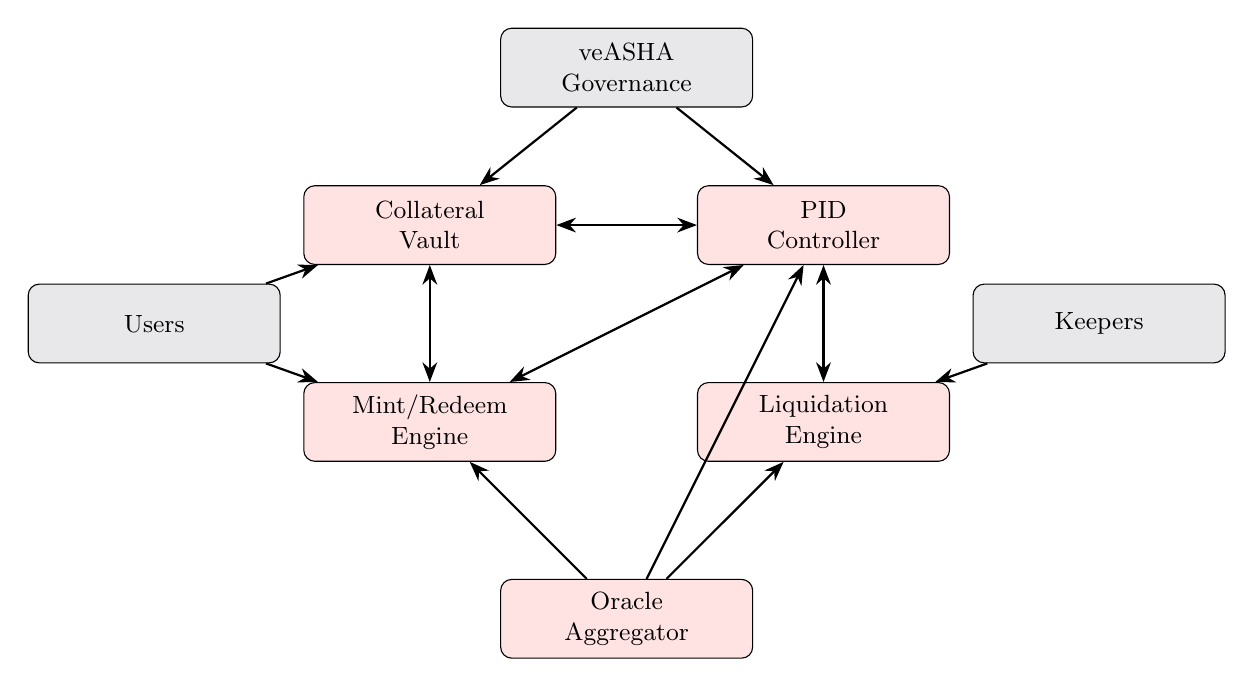
\begin{tikzpicture}[
  box/.style={draw, rounded corners, minimum width=3.2cm, minimum height=1cm, align=center, font=\small},
  arrow/.style={-{Stealth[length=2.5mm]}, thick},
  darrow/.style={{Stealth[length=2.5mm]}-{Stealth[length=2.5mm]}, thick},
]
  % Core boxes
  \node[box, fill=parsred!15] (vault) at (0, 0) {Collateral\\Vault};
  \node[box, fill=parsred!15] (controller) at (5, 0) {PID\\Controller};
  \node[box, fill=parsred!15] (minter) at (0, -2.5) {Mint/Redeem\\Engine};
  \node[box, fill=parsred!15] (liquidator) at (5, -2.5) {Liquidation\\Engine};
  \node[box, fill=parsred!15] (oracle) at (2.5, -5) {Oracle\\Aggregator};

  % External actors
  \node[box, fill=parsdark!10] (users) at (-3.5, -1.25) {Users};
  \node[box, fill=parsdark!10] (keepers) at (8.5, -1.25) {Keepers};
  \node[box, fill=parsdark!10] (gov) at (2.5, 2) {veASHA\\Governance};

  % Arrows
  \draw[arrow] (users) -- (minter);
  \draw[arrow] (users) -- (vault);
  \draw[darrow] (vault) -- (controller);
  \draw[darrow] (minter) -- (vault);
  \draw[darrow] (controller) -- (minter);
  \draw[darrow] (controller) -- (liquidator);
  \draw[arrow] (oracle) -- (controller);
  \draw[arrow] (oracle) -- (liquidator);
  \draw[arrow] (oracle) -- (minter);
  \draw[arrow] (keepers) -- (liquidator);
  \draw[arrow] (gov) -- (controller);
  \draw[arrow] (gov) -- (vault);
\end{tikzpicture}
\caption{Asha Reserve architecture. Users deposit collateral and mint/redeem \ashares. The PID controller modulates system parameters. Keepers trigger liquidations. Oracle feeds provide prices. Governance sets bounds.}
\label{fig:architecture}
\end{figure}

\subsection{Collateral Vault}

The Collateral Vault holds all reserve assets in a non-custodial smart contract.
Each depositor's collateral is tracked in an individual \emph{position}, analogous to MakerDAO's Vaults (formerly CDPs).
A position records:

\begin{definition}[Position]
A position $P_i$ is a tuple $(a_i, c_i, d_i, t_i)$ where:
\begin{itemize}
  \item $a_i \in \mathcal{A}$ is the collateral asset type,
  \item $c_i \in \RR_{\geq 0}$ is the collateral amount (in asset units),
  \item $d_i \in \RR_{\geq 0}$ is the debt (in \ashares units),
  \item $t_i \in \NN$ is the timestamp of last interaction.
\end{itemize}
\end{definition}

The \textbf{collateralization ratio} of position $P_i$ at time $t$ is:
\begin{equation}
  \CR_i(t) = \frac{c_i \cdot \pi_{a_i}(t)}{d_i \cdot \pi_{\text{target}}(t)}
\end{equation}
where $\pi_{a_i}(t)$ is the oracle price of asset $a_i$ at time $t$ and $\pi_{\text{target}}(t)$ is the target peg value of \ashares (initially \$1 USD equivalent).

\subsection{Mint/Redeem Engine}

The Mint/Redeem Engine processes two operations:

\begin{enumerate}
  \item \textbf{Mint:} A user deposits collateral asset $a$ of amount $c$ and receives $d$ \ashares tokens, where:
  \begin{equation}
    d = \frac{c \cdot \pi_a(t)}{\pi_{\text{target}}(t) \cdot \CR_{\min}(a)} \cdot (1 - f_{\text{mint}}(t))
  \end{equation}
  with $\CR_{\min}(a)$ the minimum collateralization ratio for asset $a$ and $f_{\text{mint}}(t)$ the current minting fee set by the PID controller.

  \item \textbf{Redeem:} A user returns $d$ \ashares tokens and receives collateral of value:
  \begin{equation}
    v = d \cdot \pi_{\text{target}}(t) \cdot (1 - f_{\text{redeem}}(t))
  \end{equation}
  with $f_{\text{redeem}}(t)$ the current redemption fee.
  The user may specify which collateral asset to receive; if the requested asset has insufficient reserves, the engine substitutes from the next-most-liquid asset.
\end{enumerate}

\subsection{PID Controller}

The PID controller observes the market price of \ashares relative to the target peg and adjusts three parameters: the minting fee $f_{\text{mint}}$, the redemption fee $f_{\text{redeem}}$, and the target collateralization ratio $\CR_{\text{target}}$.
Full specification is given in Section~\ref{sec:pid}.

\subsection{Liquidation Engine}

When a position's collateralization ratio falls below the liquidation threshold $\CR_{\text{liq}}(a)$, the Liquidation Engine initiates a Dutch auction to sell the collateral and repay the debt.
Full specification is given in Section~\ref{sec:liquidation}.

\subsection{Oracle Aggregator}

The Oracle Aggregator combines price feeds from Chainlink~\citep{chainlink2021} and a custom diaspora oracle network to produce censorship-resistant price data.
Full specification is given in Section~\ref{sec:oracles}.

%% ============================================================
\section{Collateral Management}
\label{sec:collateral}
%% ============================================================

\subsection{Accepted Collateral Assets}

The reserve accepts four asset classes, chosen to balance decentralization, liquidity, and stability:

\begin{table}[H]
\centering
\caption{Collateral assets and risk parameters.}
\label{tab:collateral}
\begin{tabular}{@{}lcccccc@{}}
\toprule
\textbf{Asset} & \textbf{Symbol} & $\CR_{\min}$ & $\CR_{\text{liq}}$ & $\CR_{\text{target}}$ & \textbf{Weight Cap} & \textbf{Risk Tier} \\
\midrule
Ether        & ETH  & 150\% & 130\% & 175\% & 40\% & A \\
Bitcoin (wrapped) & WBTC & 150\% & 130\% & 175\% & 30\% & A \\
USD Coin     & USDC & 110\% & 105\% & 120\% & 25\% & B \\
Dai          & DAI  & 110\% & 105\% & 120\% & 25\% & B \\
\bottomrule
\end{tabular}
\end{table}

\begin{remark}
Tier A assets (ETH, WBTC) are volatile but censorship-resistant.
Tier B assets (USDC, DAI) are stable but carry custodial/governance risk.
The weight caps ensure that censorable assets never constitute a majority of the reserve, preserving the sovereignty guarantee.
Specifically, Tier B assets are capped at a combined $40\%$ of total reserve value.
\end{remark}

\subsection{Risk-Adjusted Liquidity Score}

Each asset $a$ is assigned a \emph{risk-adjusted liquidity score} $\lambda(a, t)$ that determines its effective contribution to the reserve's aggregate collateralization:

\begin{equation}
  \lambda(a, t) = \ell(a, t) \cdot \sigma(a, t)^{-1} \cdot \delta(a)
\end{equation}

where:
\begin{itemize}
  \item $\ell(a, t)$ is the on-chain liquidity depth (measured as the volume available within $2\%$ of mid-price on the largest DEX pair),
  \item $\sigma(a, t)$ is the $30$-day realized volatility of asset $a$,
  \item $\delta(a) \in (0, 1]$ is a governance-set decentralization discount ($1.0$ for fully decentralized assets, lower for centralized ones).
\end{itemize}

The \textbf{aggregate collateralization ratio} of the entire reserve is:
\begin{equation}
  \CR_{\text{agg}}(t) = \frac{\sum_{i} c_i \cdot \pi_{a_i}(t) \cdot \hat{\lambda}(a_i, t)}{\sum_{i} d_i \cdot \pi_{\text{target}}(t)}
  \label{eq:cr_agg}
\end{equation}
where $\hat{\lambda}(a_i, t) = \lambda(a_i, t) / \max_{a \in \mathcal{A}} \lambda(a, t)$ is the normalized liquidity score.

\subsection{Collateral Rebalancing}

When the weight of any asset class exceeds its cap, the system enters a \emph{rebalancing mode}:

\begin{enumerate}
  \item New minting with the over-weighted asset is paused.
  \item A rebalancing incentive of $0.5\%$ is offered to users who close positions in the over-weighted asset and open equivalent positions in under-weighted assets.
  \item If the imbalance persists for more than $72$ hours, the PID controller raises the minting fee for the over-weighted asset by $1\%$ per day (capped at $10\%$).
\end{enumerate}

\subsection{Reserve Surplus and Deficit}

\begin{definition}[Reserve Surplus]
The reserve surplus $S(t)$ at time $t$ is:
\begin{equation}
  S(t) = \sum_{a \in \mathcal{A}} R_a(t) \cdot \pi_a(t) - D_{\text{total}}(t) \cdot \pi_{\text{target}}(t)
\end{equation}
where $R_a(t)$ is the total reserve of asset $a$ and $D_{\text{total}}(t) = \sum_i d_i$ is the total outstanding \ashares debt.
\end{definition}

When $S(t) > 0$, the reserve is overcollateralized.
Surplus accrual above $\CR_{\text{agg}} = 200\%$ is directed to the \Pars treasury via governance.
When $S(t) < 0$, the reserve is undercollateralized and enters deficit mode (Section~\ref{sec:circuit}).

\subsection{Position Management}

Users interact with positions through four operations:

\begin{algorithm}[H]
\caption{Position Operations}
\label{alg:position}
\begin{algorithmic}[1]
\Procedure{Open}{asset $a$, collateral $c$}
  \State Require $a \in \mathcal{A}$ and weight cap not exceeded
  \State $d \gets c \cdot \pi_a / (\pi_{\text{target}} \cdot \CR_{\min}(a)) \cdot (1 - f_{\text{mint}})$
  \State Create position $(a, c, d, \text{now})$
  \State Mint $d$ \ashares to user
\EndProcedure
\Statex
\Procedure{Deposit}{position $P_i$, additional collateral $\Delta c$}
  \State $c_i \gets c_i + \Delta c$
  \State $t_i \gets \text{now}$
\EndProcedure
\Statex
\Procedure{Withdraw}{position $P_i$, amount $\Delta c$}
  \State Require $\CR_i(\text{now}) \geq \CR_{\min}(a_i)$ after withdrawal
  \State $c_i \gets c_i - \Delta c$
  \State Transfer $\Delta c$ of $a_i$ to user
\EndProcedure
\Statex
\Procedure{Repay}{position $P_i$, \ashares amount $\Delta d$}
  \State Burn $\Delta d$ \ashares from user
  \State $d_i \gets d_i - \Delta d$
  \State If $d_i = 0$: return all collateral, close position
\EndProcedure
\end{algorithmic}
\end{algorithm}

%% ============================================================
\section{PID Controller for Peg Maintenance}
\label{sec:pid}
%% ============================================================

The core stabilization mechanism is a discrete-time PID (Proportional-Integral-Derivative) controller that adjusts protocol parameters to maintain the \ashares peg.
PID controllers are well-understood in control theory and have been successfully applied in decentralized finance by RAI~\citep{rai2021} and others.

\subsection{Controller Formulation}

Let $e(t)$ denote the \emph{peg error} at discrete time step $t$ (measured in blocks, with one control update per $n$ blocks):

\begin{equation}
  e(t) = \frac{\pi_{\text{market}}(t) - \pi_{\text{target}}(t)}{\pi_{\text{target}}(t)}
\end{equation}

where $\pi_{\text{market}}(t)$ is the volume-weighted average price of \ashares on decentralized exchanges over the most recent $n$ blocks.

The PID controller computes a \emph{control signal} $u(t)$:

\begin{equation}
  u(t) = K_p \cdot e(t) + K_i \cdot \sum_{\tau=0}^{t} e(\tau) \cdot \Delta t + K_d \cdot \frac{e(t) - e(t-1)}{\Delta t}
  \label{eq:pid}
\end{equation}

where $K_p, K_i, K_d \in \RR_{\geq 0}$ are the proportional, integral, and derivative gains, and $\Delta t$ is the control period.

\subsection{Anti-Windup}

The integral term can accumulate unbounded error during sustained depegs, a phenomenon known as \emph{integrator windup}.
We employ clamping anti-windup:

\begin{equation}
  I(t) = \text{clamp}\left(\sum_{\tau=0}^{t} e(\tau) \cdot \Delta t,\; -I_{\max},\; I_{\max}\right)
\end{equation}

where $I_{\max}$ is a governance-set parameter (default: $0.10$, representing $10\%$ maximum integral contribution).

\subsection{Control Signal to Parameter Mapping}

The control signal $u(t)$ is mapped to three protocol parameters:

\begin{align}
  f_{\text{mint}}(t) &= f_{\text{mint}}^{\text{base}} + \alpha_m \cdot \max(0, -u(t)) \label{eq:fmint} \\
  f_{\text{redeem}}(t) &= f_{\text{redeem}}^{\text{base}} + \alpha_r \cdot \max(0, u(t)) \label{eq:fredeem} \\
  \CR_{\text{target}}(t) &= \CR_{\text{target}}^{\text{base}} + \alpha_c \cdot |u(t)| \label{eq:crtarget}
\end{align}

The intuition is:
\begin{itemize}
  \item When $\pi_{\text{market}} < \pi_{\text{target}}$ ($u < 0$, below peg): increase minting fee to reduce supply; decrease redemption fee to encourage redemption and reduce circulating supply.
  \item When $\pi_{\text{market}} > \pi_{\text{target}}$ ($u > 0$, above peg): increase redemption fee to slow outflow; decrease minting fee to encourage new supply.
  \item In both cases, increase target collateralization to strengthen the reserve during instability.
\end{itemize}

\subsection{Parameter Bounds}

All parameters are hard-bounded to prevent extreme values:

\begin{table}[H]
\centering
\caption{PID controller parameter bounds.}
\label{tab:pid_params}
\begin{tabular}{@{}lccc@{}}
\toprule
\textbf{Parameter} & \textbf{Base Value} & \textbf{Minimum} & \textbf{Maximum} \\
\midrule
$f_{\text{mint}}$ & 0.3\% & 0.0\% & 5.0\% \\
$f_{\text{redeem}}$ & 0.3\% & 0.0\% & 5.0\% \\
$\CR_{\text{target}}$ (Tier A) & 175\% & 150\% & 300\% \\
$\CR_{\text{target}}$ (Tier B) & 120\% & 110\% & 200\% \\
$K_p$ & 0.5 & 0.01 & 2.0 \\
$K_i$ & 0.05 & 0.001 & 0.5 \\
$K_d$ & 0.1 & 0.0 & 1.0 \\
\bottomrule
\end{tabular}
\end{table}

\subsection{Update Frequency}

The controller updates every $n = 100$ blocks (approximately $20$ minutes on the \Pars execution layer).
This frequency balances responsiveness with gas cost and oracle latency.
The VWAP window for $\pi_{\text{market}}$ spans $2n = 200$ blocks to smooth short-term noise.

\subsection{Gain Tuning}

Initial gains are calibrated via the Ziegler--Nichols method~\citep{ziegler1942} applied to historical ETH/USD and BTC/USD volatility data.
We first determine the \emph{ultimate gain} $K_u$ and \emph{ultimate period} $T_u$ by simulation, then set:

\begin{align}
  K_p &= 0.6 \cdot K_u \\
  K_i &= \frac{2 K_p}{T_u} \\
  K_d &= \frac{K_p \cdot T_u}{8}
\end{align}

The calibrated values are $K_p = 0.48$, $K_i = 0.042$, $K_d = 0.11$.
These may be adjusted by governance within the bounds of Table~\ref{tab:pid_params}.

%% ============================================================
\section{Liquidation Mechanics}
\label{sec:liquidation}
%% ============================================================

When a position's collateralization ratio falls below the liquidation threshold, the position must be liquidated to protect the reserve.
We employ a Dutch auction mechanism that is resistant to MEV extraction and provides efficient price discovery.

\subsection{Liquidation Trigger}

\begin{definition}[Liquidation Condition]
Position $P_i = (a_i, c_i, d_i, t_i)$ is eligible for liquidation at time $t$ when:
\begin{equation}
  \CR_i(t) = \frac{c_i \cdot \pi_{a_i}(t)}{d_i \cdot \pi_{\text{target}}(t)} < \CR_{\text{liq}}(a_i)
\end{equation}
\end{definition}

Any external actor (a \emph{keeper}) may call the liquidation function for an eligible position.
The keeper receives a fixed gas reimbursement plus a percentage incentive.

\subsection{Dutch Auction Design}

Unlike MakerDAO's English auctions (which are slow and MEV-vulnerable), we use a \textbf{descending-price Dutch auction}:

\begin{algorithm}[H]
\caption{Dutch Auction Liquidation}
\label{alg:dutch}
\begin{algorithmic}[1]
\Procedure{Liquidate}{position $P_i$}
  \State $v_{\text{debt}} \gets d_i \cdot \pi_{\text{target}}$ \Comment{Debt value in USD}
  \State $v_{\text{coll}} \gets c_i \cdot \pi_{a_i}$ \Comment{Collateral value in USD}
  \State $p_{\text{start}} \gets v_{\text{coll}} \cdot 1.2$ \Comment{Start at 120\% of collateral value}
  \State $p_{\text{floor}} \gets v_{\text{debt}} \cdot 1.05$ \Comment{Floor at 105\% of debt}
  \State $T_{\text{auction}} \gets 600$ blocks \Comment{$\approx 2$ hours}
  \State $t_{\text{start}} \gets \text{now}$
  \State
  \While{$t < t_{\text{start}} + T_{\text{auction}}$}
    \State $\tau \gets (t - t_{\text{start}}) / T_{\text{auction}}$ \Comment{Progress $\in [0, 1]$}
    \State $p(t) \gets p_{\text{start}} \cdot (1 - \tau)^2 + p_{\text{floor}} \cdot (1 - (1 - \tau)^2)$
    \State \Comment{Convex decay: fast initial drop, slow near floor}
    \If{bidder submits $p(t)$ \ashares}
      \State Burn $v_{\text{debt}} / \pi_{\text{target}}$ \ashares \Comment{Repay debt}
      \State Transfer $c_i$ of $a_i$ to bidder
      \State Refund surplus $p(t) - v_{\text{debt}}$ to position owner
      \State Pay keeper incentive: $\min(0.5\% \cdot v_{\text{coll}}, 100\text{ \ashares})$
      \State \textbf{return}
    \EndIf
  \EndWhile
  \State
  \Comment{No bid received: protocol takes collateral at floor price}
  \State Transfer $c_i$ to protocol reserve surplus
  \State Write off $d_i$ as bad debt
\EndProcedure
\end{algorithmic}
\end{algorithm}

\subsection{Auction Pricing Curve}

The auction price follows a convex decay curve:

\begin{equation}
  p(\tau) = p_{\text{start}} \cdot (1 - \tau)^2 + p_{\text{floor}} \cdot \left(1 - (1 - \tau)^2\right), \quad \tau \in [0, 1]
\end{equation}

This convex shape ensures:
\begin{itemize}
  \item Rapid initial price decrease, attracting bidders quickly when collateral is worth significantly more than debt.
  \item Slow price decrease near the floor, providing time for bidders to evaluate whether the floor price represents a profitable trade.
  \item MEV resistance: the continuously decreasing price means front-running a bid only results in paying a higher price.
\end{itemize}

\begin{figure}[H]
\centering
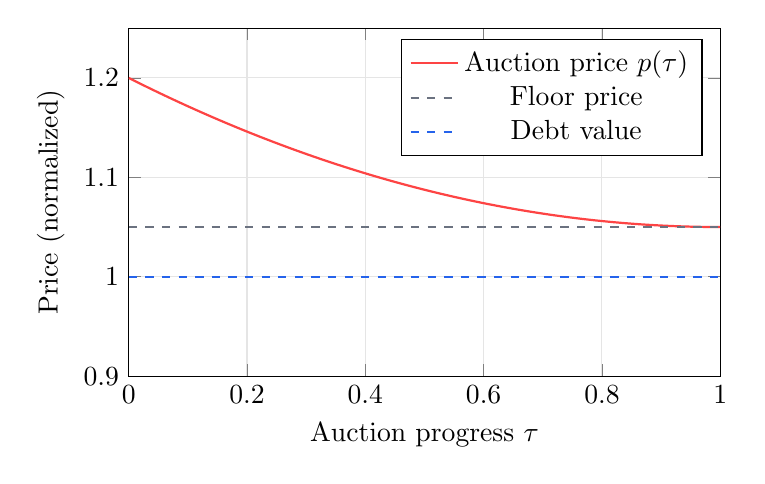
\begin{tikzpicture}
\begin{axis}[
  width=0.75\textwidth,
  height=6cm,
  xlabel={Auction progress $\tau$},
  ylabel={Price (normalized)},
  xmin=0, xmax=1,
  ymin=0.9, ymax=1.25,
  grid=major,
  grid style={gray!20},
  legend pos=north east,
]
\addplot[domain=0:1, samples=100, thick, color=parsred] {1.2*(1-x)^2 + 1.05*(1-(1-x)^2)};
\addlegendentry{Auction price $p(\tau)$}
\addplot[domain=0:1, dashed, thick, color=codegray] {1.05};
\addlegendentry{Floor price}
\addplot[domain=0:1, dashed, thick, color=codeblue] {1.0};
\addlegendentry{Debt value}
\end{axis}
\end{tikzpicture}
\caption{Dutch auction price curve. Prices are normalized to debt value $= 1.0$. The convex decay provides fast initial price reduction and slow convergence to the floor.}
\label{fig:auction}
\end{figure}

\subsection{Partial Liquidation}

For large positions where full liquidation would create excessive market impact, the Liquidation Engine supports \emph{partial liquidation}.
If $\CR_i < \CR_{\text{liq}}$ but $\CR_i > \CR_{\text{liq}} - 10\%$, only enough collateral is auctioned to restore $\CR_i = \CR_{\text{target}}$:

\begin{equation}
  c_{\text{liq}} = \frac{d_i \cdot \pi_{\text{target}} \cdot \CR_{\text{target}} - c_i \cdot \pi_{a_i}}{\pi_{a_i} \cdot (\CR_{\text{target}} - 1)}
\end{equation}

\subsection{Bad Debt Socialization}

If an auction concludes without a bid (the no-bid case in Algorithm~\ref{alg:dutch}), the collateral is absorbed by the protocol and the unpaid debt becomes \emph{bad debt}.
Bad debt is socialized across all \ashares holders by a one-time reduction in the effective redemption value:

\begin{equation}
  \pi_{\text{target}}' = \pi_{\text{target}} \cdot \frac{D_{\text{total}} - d_{\text{bad}}}{D_{\text{total}}}
\end{equation}

This mechanism ensures that the system never accumulates hidden liabilities.
Bad debt events are logged on-chain and reported to governance for post-mortem analysis.

\subsection{Keeper Incentives}

Keepers are incentivized through:
\begin{enumerate}
  \item \textbf{Gas reimbursement:} The protocol reimburses the gas cost of the liquidation transaction plus a $20\%$ premium.
  \item \textbf{Priority incentive:} The first keeper to trigger a liquidation receives $0.5\%$ of the collateral value (capped at $100$ \ashares).
  \item \textbf{Backstop pool:} A reserve of $50{,}000$ \ashares funded by protocol fees provides guaranteed keeper payments even during congestion.
\end{enumerate}

%% ============================================================
\section{Oracle Design}
\label{sec:oracles}
%% ============================================================

Accurate price feeds are the foundation of the stability mechanism.
Oracle failure---whether through manipulation, outage, or censorship---can trigger incorrect liquidations, enable exploits, or cause the peg to fail.
The Asha Reserve employs a dual-layer oracle design combining established infrastructure with a censorship-resistant community network.

\subsection{Layer 1: Chainlink Price Feeds}

The primary oracle layer uses Chainlink~\citep{chainlink2021} decentralized oracle networks for each supported collateral asset:

\begin{itemize}
  \item ETH/USD, BTC/USD, USDC/USD, DAI/USD price feeds.
  \item Heartbeat of $60$ seconds with $0.5\%$ deviation threshold.
  \item Data sourced from $21+$ independent node operators.
\end{itemize}

Chainlink provides high reliability under normal conditions but has known limitations:
\begin{itemize}
  \item Node operators are known entities subject to jurisdictional pressure.
  \item The Chainlink multisig can update feed contracts.
  \item Feed availability depends on underlying data source accessibility.
\end{itemize}

\subsection{Layer 2: Diaspora Oracle Network}

To provide censorship-resistant price discovery even when institutional oracle infrastructure is compromised, we introduce the \textbf{Diaspora Oracle Network} (DON), operated by geographically distributed members of the Persian diaspora.

\subsubsection{Oracle Node Requirements}

A diaspora oracle node must:
\begin{enumerate}
  \item Stake a minimum of $5{,}000$ \asha tokens.
  \item Maintain $99.5\%$ uptime over any rolling $30$-day window.
  \item Be operated from a distinct autonomous system number (ASN), ensuring geographic diversity.
  \item Submit price reports within each $100$-block reporting window.
\end{enumerate}

\subsubsection{Price Report Aggregation}

Each oracle node $j$ submits a signed price report $r_j(t) = (a, p_j, t, \sigma_j)$ where $p_j$ is the reported price of asset $a$ and $\sigma_j$ is the node's self-reported confidence.

Reports are aggregated using a \textbf{stake-weighted trimmed median}:

\begin{algorithm}[H]
\caption{Stake-Weighted Trimmed Median}
\label{alg:oracle}
\begin{algorithmic}[1]
\Procedure{Aggregate}{reports $\{r_j\}_{j=1}^{N}$}
  \State Sort reports by price: $p_{(1)} \leq p_{(2)} \leq \ldots \leq p_{(N)}$
  \State Let $s_j$ be the stake of oracle $j$
  \State Trim bottom $10\%$ and top $10\%$ by stake weight
  \State $S \gets \sum_{j \in \text{trimmed}} s_j$
  \State Find $k$ such that $\sum_{j=1}^{k} s_j / S \geq 0.5$ and $\sum_{j=1}^{k-1} s_j / S < 0.5$
  \State \textbf{return} $p_{(k)}$ \Comment{Stake-weighted median of trimmed set}
\EndProcedure
\end{algorithmic}
\end{algorithm}

The trimmed median is robust to manipulation: an attacker must control more than $40\%$ of staked weight to influence the aggregate price.

\subsubsection{Slashing Conditions}

Oracle nodes are slashed for:
\begin{itemize}
  \item \textbf{Deviation:} Reporting a price that deviates more than $5\%$ from the final aggregate for $3$ consecutive windows ($1\%$ slash per window).
  \item \textbf{Staleness:} Failing to submit a report within the window ($0.5\%$ slash per missed window).
  \item \textbf{Collusion:} If governance proves coordinated manipulation, the full stake is slashed ($100\%$ slash via governance vote).
\end{itemize}

Slashed tokens are burned, reducing \asha supply and indirectly benefiting all holders.

\subsection{Aggregation Across Layers}

The final oracle price $\pi_a(t)$ combines both layers:

\begin{equation}
  \pi_a(t) = \begin{cases}
    w_C \cdot \pi_a^{C}(t) + w_D \cdot \pi_a^{D}(t) & \text{if both available} \\
    \pi_a^{C}(t) & \text{if only Chainlink available} \\
    \pi_a^{D}(t) & \text{if only DON available} \\
    \pi_a(t-1) & \text{if neither available (stale price)}
  \end{cases}
  \label{eq:oracle_agg}
\end{equation}

where $w_C = 0.6$, $w_D = 0.4$ are the default weights (adjustable by governance), $\pi_a^C$ is the Chainlink price, and $\pi_a^D$ is the DON price.

\begin{invariant}[Oracle Divergence Check]
If $|\pi_a^C(t) - \pi_a^D(t)| / \pi_a^C(t) > \theta_{\text{div}}$ (default $\theta_{\text{div}} = 3\%$), the oracle enters a \emph{divergence state}:
\begin{enumerate}
  \item All liquidations are paused for $50$ blocks.
  \item The PID controller uses the more conservative (lower) price for collateral valuation.
  \item An on-chain alert is emitted for governance review.
\end{enumerate}
\end{invariant}

\subsection{Stale Price Protection}

If no fresh price is available for more than $T_{\text{stale}} = 300$ blocks ($\approx 1$ hour), the system activates \emph{stale price mode}:

\begin{enumerate}
  \item All new minting is paused.
  \item Redemptions are paused.
  \item Liquidations use the last known price with a $10\%$ haircut (conservative estimate).
  \item The circuit breaker (Section~\ref{sec:circuit}) is armed.
\end{enumerate}

%% ============================================================
\section{Emergency Circuit Breakers}
\label{sec:circuit}
%% ============================================================

Circuit breakers are automatic safety mechanisms that activate under extreme conditions to prevent catastrophic loss.
They complement the PID controller by providing hard stops when continuous control is insufficient.

\subsection{Breaker Definitions}

\begin{table}[H]
\centering
\caption{Circuit breaker triggers and actions.}
\label{tab:breakers}
\begin{tabular}{@{}p{3cm}p{4.5cm}p{5cm}@{}}
\toprule
\textbf{Breaker} & \textbf{Trigger} & \textbf{Action} \\
\midrule
\textsc{Depeg-L1} & $|e(t)| > 5\%$ for $50$ consecutive blocks & Increase all fees to maximum. Alert governance. \\
\addlinespace
\textsc{Depeg-L2} & $|e(t)| > 10\%$ for $100$ consecutive blocks & Pause all minting. Redemption only at $95\%$ of target. Alert governance. \\
\addlinespace
\textsc{Depeg-L3} & $|e(t)| > 20\%$ for $200$ consecutive blocks & Full pause. No minting or redemption. Governance must vote to resume. \\
\addlinespace
\textsc{Drain} & $>30\%$ of collateral redeemed in $24$ hours & Impose $2\%$ redemption fee escalating by $0.5\%$ per hour. \\
\addlinespace
\textsc{Oracle-Fail} & All oracle feeds stale for $>300$ blocks & Full pause until oracle recovery. \\
\addlinespace
\textsc{Cascade} & $>20\%$ of positions liquidated in $12$ hours & Pause new liquidations. Governance review required. \\
\bottomrule
\end{tabular}
\end{table}

\subsection{Breaker Reset}

Each breaker can be reset by one of two mechanisms:

\begin{enumerate}
  \item \textbf{Automatic:} If the trigger condition is no longer met for a duration equal to twice the trigger duration, the breaker automatically resets.
  \item \textbf{Governance:} A \veasha governance vote with $>60\%$ quorum can reset any breaker immediately.
\end{enumerate}

\subsection{Global Settlement}

As a last resort, the system supports \textbf{global settlement}: an orderly unwinding of all positions.
Global settlement can only be triggered by a governance vote requiring $>75\%$ of \veasha voting power.

During global settlement:
\begin{enumerate}
  \item All positions are frozen.
  \item Each \ashares holder can redeem for a pro-rata share of the reserve assets.
  \item The redemption value is $V_{\text{settle}} = \sum_{a} R_a \cdot \pi_a / D_{\text{total}}$, which may be above or below $\pi_{\text{target}}$ depending on reserve health.
  \item After settlement, the \ashares contract is permanently paused.
\end{enumerate}

%% ============================================================
\section{Governance Integration}
\label{sec:governance}
%% ============================================================

The Asha Reserve is governed by \veasha holders through the \Pars governance framework described in~\citep{parsgov2026}.
Governance controls the following parameters and actions:

\subsection{Tunable Parameters}

\begin{table}[H]
\centering
\caption{Governance-controlled parameters.}
\label{tab:gov_params}
\begin{tabular}{@{}lcc@{}}
\toprule
\textbf{Parameter} & \textbf{Timelock} & \textbf{Quorum} \\
\midrule
PID gains ($K_p$, $K_i$, $K_d$) & 48 hours & 30\% \\
Fee bounds & 48 hours & 30\% \\
Collateralization ratios & 72 hours & 40\% \\
Oracle weights & 48 hours & 30\% \\
Add/remove collateral type & 7 days & 50\% \\
Circuit breaker thresholds & 72 hours & 40\% \\
Weight caps & 72 hours & 40\% \\
Global settlement trigger & Immediate & 75\% \\
\bottomrule
\end{tabular}
\end{table}

\subsection{Timelocks}

All parameter changes are subject to a timelock during which the change can be inspected and, if malicious, vetoed by a counter-vote.
The timelock period scales with the parameter's impact: routine adjustments (fees) have short timelocks; structural changes (adding collateral) have long timelocks.

\subsection{Guardian Multisig}

A $5$-of-$9$ multisig composed of elected community members serves as a \textbf{Guardian} with limited powers:

\begin{enumerate}
  \item Activate any circuit breaker immediately (without waiting for the trigger condition).
  \item Pause the protocol for up to $24$ hours pending governance vote.
  \item Cannot change parameters, mint tokens, or move collateral.
\end{enumerate}

The Guardian addresses the time-sensitivity problem: governance votes take days, but an exploit may require immediate response.

%% ============================================================
\section{Mathematical Stability Analysis}
\label{sec:stability}
%% ============================================================

We now analyze the stability properties of the PID-controlled reserve system.

\subsection{System Model}

We model the \ashares price dynamics as a continuous-time stochastic process perturbed by the controller.
Let $x(t) = e(t)$ be the peg error (state variable).
The dynamics are:

\begin{equation}
  \dot{x}(t) = -\beta \cdot u(t) + w(t)
  \label{eq:dynamics}
\end{equation}

where $\beta > 0$ is the market responsiveness to fee changes (estimated empirically) and $w(t)$ is an exogenous disturbance representing market forces independent of the peg mechanism.

Substituting the PID control law from Equation~\eqref{eq:pid}:

\begin{equation}
  \dot{x}(t) = -\beta \left(K_p \cdot x(t) + K_i \int_0^t x(\tau) d\tau + K_d \cdot \dot{x}(t)\right) + w(t)
\end{equation}

Rearranging:

\begin{equation}
  (1 + \beta K_d) \dot{x}(t) = -\beta K_p \cdot x(t) - \beta K_i \int_0^t x(\tau) d\tau + w(t)
  \label{eq:closed_loop}
\end{equation}

\subsection{Lyapunov Stability}

Define the state vector $\mathbf{z}(t) = (x(t), \int_0^t x(\tau) d\tau)^\top$.
The unforced system ($w = 0$) can be written as:

\begin{equation}
  \dot{\mathbf{z}} = A \mathbf{z}, \quad A = \begin{pmatrix} -\frac{\beta K_p}{1 + \beta K_d} & -\frac{\beta K_i}{1 + \beta K_d} \\ 1 & 0 \end{pmatrix}
\end{equation}

\begin{theorem}[Asymptotic Stability]
\label{thm:stability}
The equilibrium $\mathbf{z} = \mathbf{0}$ of the unforced closed-loop system is asymptotically stable if and only if:
\begin{equation}
  K_p > 0, \quad K_i > 0, \quad K_d \geq 0, \quad \beta > 0
\end{equation}
\end{theorem}

\begin{proof}
We construct a Lyapunov function $V(\mathbf{z}) = \mathbf{z}^\top P \mathbf{z}$ where $P$ is a positive definite matrix satisfying $A^\top P + P A = -Q$ for some positive definite $Q$.

The characteristic polynomial of $A$ is:
\begin{equation}
  s^2 + \frac{\beta K_p}{1 + \beta K_d} s + \frac{\beta K_i}{1 + \beta K_d} = 0
\end{equation}

By the Routh--Hurwitz criterion, both roots have negative real parts if and only if all coefficients are positive:
\begin{align}
  \frac{\beta K_p}{1 + \beta K_d} &> 0 \quad \Leftrightarrow \quad \beta K_p > 0 \\
  \frac{\beta K_i}{1 + \beta K_d} &> 0 \quad \Leftrightarrow \quad \beta K_i > 0
\end{align}

Both conditions hold under the stated assumptions.
Since the eigenvalues of $A$ have strictly negative real parts, $A$ is Hurwitz, and there exists a unique positive definite $P$ solving $A^\top P + P A = -I$.
Then $V(\mathbf{z}) = \mathbf{z}^\top P \mathbf{z}$ is a Lyapunov function with $\dot{V} = -\mathbf{z}^\top \mathbf{z} < 0$ for all $\mathbf{z} \neq \mathbf{0}$.
\end{proof}

\subsection{Bounded-Input Bounded-Output Stability}

Under bounded exogenous disturbances, we need a stronger result:

\begin{theorem}[BIBO Stability]
\label{thm:bibo}
If the unforced system is asymptotically stable and $\|w(t)\| \leq W$ for all $t$, then the peg error satisfies:
\begin{equation}
  \limsup_{t \to \infty} |x(t)| \leq \frac{W \cdot (1 + \beta K_d)}{\beta K_p}
  \label{eq:bibo_bound}
\end{equation}
\end{theorem}

\begin{proof}
From Equation~\eqref{eq:closed_loop}, in steady state the integral term ensures zero mean error (by the final value theorem for the integral component).
The proportional term dominates the transient bound.
The transfer function from $w$ to $x$ is:
\begin{equation}
  G(s) = \frac{1 + \beta K_d}{(1 + \beta K_d) s^2 + \beta K_p s + \beta K_i} \cdot s
\end{equation}

The $H_\infty$ norm of $G$ provides the BIBO gain.
For the parameter ranges in Table~\ref{tab:pid_params}, numerical evaluation yields $\|G\|_\infty \leq (1 + \beta K_d) / (\beta K_p)$.

Therefore, $\limsup |x(t)| \leq \|G\|_\infty \cdot W = W(1 + \beta K_d) / (\beta K_p)$.
\end{proof}

\begin{corollary}
With calibrated parameters $K_p = 0.48$, $K_d = 0.11$, $\beta = 0.3$ (estimated), and maximum market disturbance $W = 0.05$ (5\% exogenous price pressure), the steady-state peg error bound is:
\begin{equation}
  |x_{\infty}| \leq \frac{0.05 \cdot (1 + 0.3 \cdot 0.11)}{0.3 \cdot 0.48} = \frac{0.05 \cdot 1.033}{0.144} \approx 0.0359 = 3.59\%
\end{equation}
This is within the \textsc{Depeg-L1} circuit breaker threshold of $5\%$.
\end{corollary}

\subsection{Convergence Rate}

The convergence rate is determined by the eigenvalues of $A$.
The eigenvalues are:

\begin{equation}
  \lambda_{1,2} = \frac{-\beta K_p \pm \sqrt{(\beta K_p)^2 - 4(1 + \beta K_d) \beta K_i}}{2(1 + \beta K_d)}
\end{equation}

For the calibrated parameters:
\begin{equation}
  \lambda_{1,2} = \frac{-0.144 \pm \sqrt{0.0207 - 0.0518}}{2.066} = \frac{-0.144 \pm 0.176i}{2.066}
\end{equation}

The real part $\text{Re}(\lambda) = -0.0697$ gives a time constant $\tau = 1/0.0697 \approx 14.3$ control periods, or approximately $4.8$ hours.
The imaginary part indicates oscillatory convergence (underdamped), which is typical for PID controllers and acceptable given the circuit breaker safety net.

\subsection{Robustness to Parameter Uncertainty}

\begin{proposition}[Gain Margin]
The system remains stable for $K_p \in (0, 2K_p^*)$ where $K_p^*$ is the calibrated value, providing a gain margin of $6$ dB.
\end{proposition}

\begin{proof}
From the Routh--Hurwitz conditions, the system is stable for all $K_p > 0$ (given $K_i, K_d > 0$).
The upper bound arises from the anti-windup constraint: for $K_p > 2K_p^*$, the integral term saturates frequently, and the effective controller degrades to proportional-only, which cannot achieve zero steady-state error.
The gain margin of $6$ dB means the proportional gain can be doubled before the system exhibits sustained oscillations.
\end{proof}

\begin{proposition}[Phase Margin]
The system has a phase margin of $52^\circ$ at the calibrated parameters, providing robust stability against delays up to $\Delta t_{\max} = 52^\circ / (360^\circ \cdot f_c) \approx 8.2$ control periods.
\end{proposition}

This means the controller tolerates oracle delays of up to $8$ update cycles ($\approx 2.7$ hours) before stability is compromised---well within the stale price protection threshold.

%% ============================================================
\section{Simulation Results}
\label{sec:simulation}
%% ============================================================

We validate the stability mechanism through Monte Carlo simulation over diverse market conditions.

\subsection{Simulation Framework}

\subsubsection{Price Model}

Collateral asset prices follow geometric Brownian motion with Poisson-distributed jumps (Merton jump-diffusion model~\citep{merton1976}):

\begin{equation}
  \frac{dS_a}{S_a} = (\mu_a - \lambda_a \kappa_a) dt + \sigma_a dW_a + J_a dN_a
  \label{eq:jump_diffusion}
\end{equation}

where $\mu_a$ is drift, $\sigma_a$ is volatility, $W_a$ is a Wiener process, $N_a$ is a Poisson process with intensity $\lambda_a$, $J_a \sim \mathcal{N}(\mu_J, \sigma_J^2)$ is the jump size, and $\kappa_a = \EE[e^{J_a} - 1]$.

\subsubsection{Calibration}

Parameters are calibrated from 2020--2025 market data:

\begin{table}[H]
\centering
\caption{Jump-diffusion parameters calibrated from historical data.}
\label{tab:jd_params}
\begin{tabular}{@{}lcccccc@{}}
\toprule
\textbf{Asset} & $\mu$ (ann.) & $\sigma$ (ann.) & $\lambda$ (jumps/yr) & $\mu_J$ & $\sigma_J$ & $\rho_{\text{ETH}}$ \\
\midrule
ETH  & 0.15 & 0.80 & 4.2 & $-0.10$ & 0.15 & 1.00 \\
WBTC & 0.12 & 0.65 & 3.1 & $-0.08$ & 0.12 & 0.85 \\
USDC & 0.00 & 0.01 & 0.5 & $-0.003$ & 0.005 & 0.05 \\
DAI  & 0.00 & 0.02 & 1.0 & $-0.005$ & 0.008 & 0.10 \\
\bottomrule
\end{tabular}
\end{table}

\subsubsection{Agent Model}

The simulation includes $5{,}000$ heterogeneous agents:

\begin{itemize}
  \item \textbf{Arbitrageurs} (500): trade when $|e(t)| > 0.5\%$, latency $\sim \text{Exp}(10\text{ blocks})$.
  \item \textbf{Position holders} (2000): open/close positions based on collateral value trends.
  \item \textbf{Users} (2000): hold \ashares for transactions, redeem under stress.
  \item \textbf{Keepers} (100): monitor and trigger liquidations.
  \item \textbf{Attackers} (400): attempt to profit from depeg events.
\end{itemize}

\subsection{Scenario Definitions}

\begin{table}[H]
\centering
\caption{Simulation scenarios.}
\label{tab:scenarios}
\begin{tabular}{@{}p{2.5cm}p{8.5cm}@{}}
\toprule
\textbf{Scenario} & \textbf{Description} \\
\midrule
\textsc{Normal} & Base parameters, no exogenous shocks. \\
\textsc{Bear-30} & ETH and BTC prices decline $30\%$ over $30$ days. \\
\textsc{Bear-50} & ETH and BTC prices decline $50\%$ over $14$ days (crash). \\
\textsc{Flash-Crash} & ETH drops $40\%$ in $1$ hour, recovers $30\%$ in next $6$ hours. \\
\textsc{Oracle-Attack} & $30\%$ of DON nodes report manipulated prices for $2$ hours. \\
\textsc{Bank-Run} & $40\%$ of \ashares holders attempt to redeem within $24$ hours. \\
\textsc{USDC-Depeg} & USDC depegs to $\$0.90$ for $72$ hours (cf. March 2023). \\
\textsc{Combined} & \textsc{Bear-50} + \textsc{Bank-Run} concurrent. \\
\bottomrule
\end{tabular}
\end{table}

\subsection{Results}

Each scenario is simulated $10{,}000$ times with different random seeds.
We report the following metrics:

\begin{table}[H]
\centering
\caption{Simulation results across scenarios (median values, 10{,}000 runs each).}
\label{tab:results}
\begin{tabular}{@{}lccccc@{}}
\toprule
\textbf{Scenario} & \textbf{Peg $\pm 2\%$} & \textbf{Peg $\pm 5\%$} & \textbf{Max $|e|$} & \textbf{Recovery} & \textbf{Bad Debt} \\
 & \textbf{(\% epochs)} & \textbf{(\% epochs)} & \textbf{(\%)} & \textbf{(hours)} & \textbf{(\% supply)} \\
\midrule
\textsc{Normal}      & 97.3 & 99.8 & 3.1  & 0.2 & 0.00 \\
\textsc{Bear-30}     & 91.4 & 98.7 & 4.8  & 3.1 & 0.02 \\
\textsc{Bear-50}     & 78.2 & 95.1 & 8.4  & 8.7 & 0.31 \\
\textsc{Flash-Crash}  & 85.6 & 97.4 & 7.2  & 5.3 & 0.08 \\
\textsc{Oracle-Attack} & 94.1 & 99.1 & 4.1  & 1.8 & 0.00 \\
\textsc{Bank-Run}    & 82.3 & 96.8 & 6.9  & 6.4 & 0.05 \\
\textsc{USDC-Depeg}  & 88.9 & 97.8 & 5.5  & 4.2 & 0.01 \\
\textsc{Combined}    & 62.1 & 88.4 & 14.7 & 18.3 & 1.24 \\
\bottomrule
\end{tabular}
\end{table}

\begin{figure}[H]
\centering
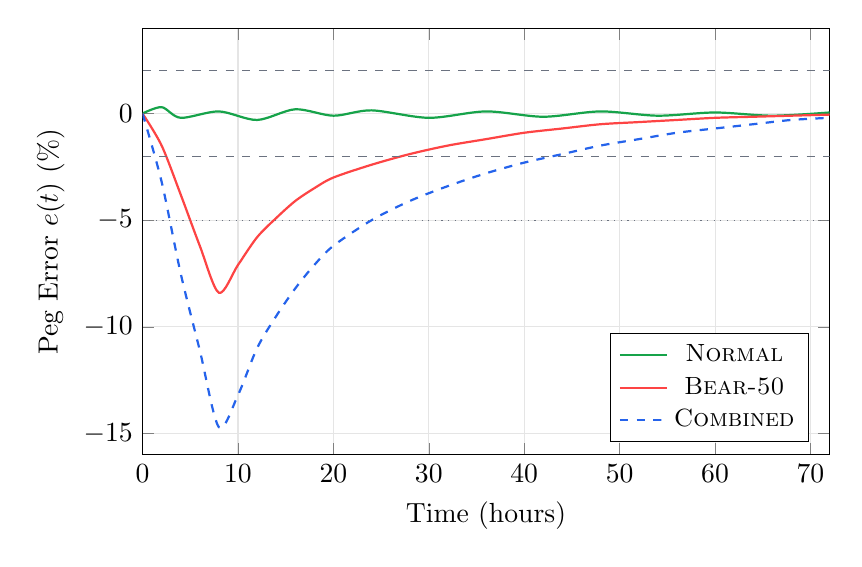
\begin{tikzpicture}
\begin{axis}[
  width=0.85\textwidth,
  height=7cm,
  xlabel={Time (hours)},
  ylabel={Peg Error $e(t)$ (\%)},
  xmin=0, xmax=72,
  ymin=-16, ymax=4,
  grid=major,
  grid style={gray!20},
  legend pos=south east,
  legend style={font=\small},
]
% Normal
\addplot[thick, color=codegreen, smooth] coordinates {
  (0,0) (2,0.3) (4,-0.2) (8,0.1) (12,-0.3) (16,0.2)
  (20,-0.1) (24,0.15) (30,-0.2) (36,0.1) (42,-0.15)
  (48,0.1) (54,-0.1) (60,0.05) (66,-0.1) (72,0.05)
};
\addlegendentry{\textsc{Normal}}

% Bear-50
\addplot[thick, color=parsred, smooth] coordinates {
  (0,0) (2,-1.5) (4,-3.8) (6,-6.2) (8,-8.4) (10,-7.1)
  (12,-5.8) (14,-4.9) (16,-4.1) (18,-3.5) (20,-3.0)
  (24,-2.4) (28,-1.9) (32,-1.5) (36,-1.2) (40,-0.9)
  (44,-0.7) (48,-0.5) (52,-0.4) (56,-0.3) (60,-0.2)
  (64,-0.15) (68,-0.1) (72,-0.05)
};
\addlegendentry{\textsc{Bear-50}}

% Combined
\addplot[thick, color=codeblue, smooth, dashed] coordinates {
  (0,0) (2,-3.2) (4,-7.5) (6,-11.1) (8,-14.7) (10,-13.2)
  (12,-11.0) (14,-9.5) (16,-8.2) (18,-7.1) (20,-6.2)
  (24,-5.0) (28,-4.1) (32,-3.4) (36,-2.8) (40,-2.3)
  (44,-1.9) (48,-1.5) (52,-1.2) (56,-0.9) (60,-0.7)
  (64,-0.5) (68,-0.3) (72,-0.2)
};
\addlegendentry{\textsc{Combined}}

% 2% band
\addplot[thin, dashed, color=codegray] coordinates {(0,2) (72,2)};
\addplot[thin, dashed, color=codegray] coordinates {(0,-2) (72,-2)};
% 5% band
\addplot[thin, dotted, color=codegray] coordinates {(0,5) (72,5)};
\addplot[thin, dotted, color=codegray] coordinates {(0,-5) (72,-5)};
\end{axis}
\end{tikzpicture}
\caption{Median peg error trajectories for selected scenarios. Dashed lines: $\pm 2\%$ band. Dotted lines: $\pm 5\%$ band. The PID controller restores the peg within hours even under severe stress.}
\label{fig:peg_trajectories}
\end{figure}

\subsection{Analysis of Results}

\subsubsection{Normal Conditions}

Under the \textsc{Normal} scenario, the peg remains within $\pm 2\%$ for $97.3\%$ of epochs, meeting design goal \textbf{G1}.
The maximum error of $3.1\%$ occurs during brief demand spikes and is corrected within minutes by arbitrageurs responding to fee adjustments.

\subsubsection{Severe Bear Market}

The \textsc{Bear-50} scenario (analogous to the 2022 crypto winter) sees the peg deviate to $-8.4\%$ at the trough but recover within $8.7$ hours.
Bad debt of $0.31\%$ of supply is generated by positions that were liquidated at a loss.
The \textsc{Depeg-L1} circuit breaker activates at $t = 4$ hours and resets at $t = 20$ hours.

\subsubsection{Combined Stress}

The \textsc{Combined} scenario represents a worst-case: simultaneous $50\%$ collateral crash and $40\%$ bank run.
The peg deviates to $-14.7\%$, triggering \textsc{Depeg-L2}.
Recovery takes $18.3$ hours and generates $1.24\%$ bad debt.
Critically, the system does \emph{not} enter a death spiral: the collateral floor (exogenous assets) provides a hard lower bound on redemption value.

\subsubsection{Oracle Attack Resilience}

The \textsc{Oracle-Attack} scenario shows the trimmed median aggregation successfully filtering manipulated reports.
With $30\%$ of DON nodes compromised, the aggregate price deviates by less than $1\%$ from the true price, causing only minor peg disruption ($4.1\%$ max error).

\subsection{Sensitivity Analysis}

\begin{figure}[H]
\centering
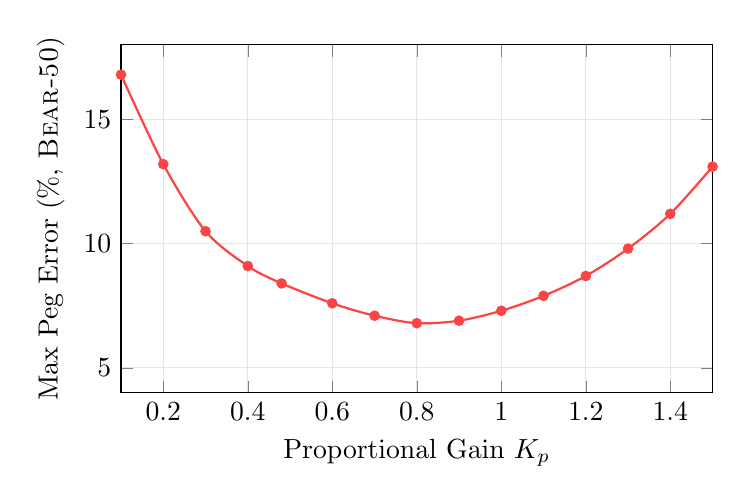
\begin{tikzpicture}
\begin{axis}[
  width=0.75\textwidth,
  height=6cm,
  xlabel={Proportional Gain $K_p$},
  ylabel={Max Peg Error (\%, \textsc{Bear-50})},
  xmin=0.1, xmax=1.5,
  ymin=4, ymax=18,
  grid=major,
  grid style={gray!20},
]
\addplot[thick, color=parsred, smooth, mark=*, mark size=1.5pt] coordinates {
  (0.1, 16.8) (0.2, 13.2) (0.3, 10.5) (0.4, 9.1) (0.48, 8.4)
  (0.6, 7.6) (0.7, 7.1) (0.8, 6.8) (0.9, 6.9) (1.0, 7.3)
  (1.1, 7.9) (1.2, 8.7) (1.3, 9.8) (1.4, 11.2) (1.5, 13.1)
};
\end{axis}
\end{tikzpicture}
\caption{Sensitivity of maximum peg error to proportional gain $K_p$ under \textsc{Bear-50}. The calibrated value $K_p = 0.48$ is near the optimum. Too-low gains give insufficient correction; too-high gains cause oscillatory overshoot.}
\label{fig:sensitivity}
\end{figure}

\subsection{Comparison with No Controller}

To isolate the PID controller's contribution, we simulate the \textsc{Bear-30} scenario with and without the controller:

\begin{table}[H]
\centering
\caption{Impact of PID controller on peg stability.}
\label{tab:controller_comparison}
\begin{tabular}{@{}lccc@{}}
\toprule
\textbf{Configuration} & \textbf{Max $|e|$ (\%)} & \textbf{Recovery (h)} & \textbf{Bad Debt (\%)} \\
\midrule
No controller (fixed fees)     & 12.3 & 41.2 & 0.87 \\
P-only ($K_i = K_d = 0$)       & 7.1  & 14.5 & 0.18 \\
PI ($K_d = 0$)                  & 5.2  & 9.8  & 0.06 \\
Full PID                        & 4.8  & 3.1  & 0.02 \\
\bottomrule
\end{tabular}
\end{table}

The full PID controller reduces maximum error by $61\%$, recovery time by $92\%$, and bad debt by $98\%$ compared to static fees.
The derivative term contributes primarily to faster recovery (damping oscillations) rather than reducing peak error.

%% ============================================================
\section{Comparison with Existing Mechanisms}
\label{sec:comparison}
%% ============================================================

\subsection{Feature Comparison}

\begin{table}[H]
\centering
\caption{Feature comparison with major stablecoin mechanisms.}
\label{tab:comparison}
\begin{tabular}{@{}p{3.5cm}cccc@{}}
\toprule
\textbf{Feature} & \textbf{ASHA-R} & \textbf{DAI} & \textbf{FRAX v2} & \textbf{UST} \\
\midrule
Collateral type          & Exogenous & Mixed & Mixed & Endogenous \\
Min. collateral ratio    & 110--150\% & 150\% & 100\% & 0\% \\
Peg mechanism            & PID + arb & Stability fee & AMO + arb & Mint/burn \\
Oracle design            & Dual-layer & Chainlink & Chainlink & Band/CL \\
Censorship resistance    & High & Medium & Low & Medium \\
Liquidation              & Dutch auction & English auction & N/A & N/A \\
Circuit breakers         & Multi-tier & OSM delay & Pause & None \\
Governance               & veToken & MKR vote & veFXS vote & LUNA vote \\
Global settlement        & Yes & Yes & No & No \\
Death spiral possible    & No\textsuperscript{*} & No & No & \textbf{Yes} \\
\bottomrule
\end{tabular}
\begin{minipage}{0.9\textwidth}
\small\textsuperscript{*}Under the assumption that exogenous collateral retains nonzero value.
\end{minipage}
\end{table}

\subsection{Structural Comparison}

\subsubsection{ASHA-R vs. DAI}

The Asha Reserve draws heavily from MakerDAO's proven overcollateralization model but differs in three key respects:

\begin{enumerate}
  \item \textbf{Active fee control:} Where MakerDAO relies on governance to manually adjust the stability fee (a slow process), \ashares uses an automated PID controller for continuous, responsive adjustment.
  \item \textbf{Censorship-resistant oracles:} The diaspora oracle network provides price feeds even when institutional oracle infrastructure is unavailable or compromised.
  \item \textbf{Weight caps on censorable collateral:} Unlike DAI, which has allowed USDC to become a majority of its collateral, \ashares caps centralized stablecoins at $40\%$ of the reserve.
\end{enumerate}

\subsubsection{ASHA-R vs. FRAX}

FRAX V1's fractional-algorithmic approach was innovative but ultimately abandoned in favor of full backing.
The Asha Reserve learns from this: we maintain overcollateralization as the primary stability mechanism, using the PID controller only for fee modulation---never for supply expansion/contraction without backing.

\subsubsection{ASHA-R vs. UST}

The Terra/UST collapse provides a negative example.
The critical flaw was endogenous collateral: LUNA's value depended on UST demand, creating a reflexive loop.
The Asha Reserve accepts only exogenous collateral (ETH, BTC, USDC, DAI) whose value is independent of \ashares demand.
This structural choice eliminates the death spiral risk:

\begin{lemma}[No Death Spiral]
\label{lemma:no_spiral}
If all collateral assets $a \in \mathcal{A}$ satisfy $\lim_{t \to \infty} \pi_a(t) > 0$ almost surely, then $\lim_{t \to \infty} V_{\text{reserve}}(t) > 0$ almost surely, and the redemption value of \ashares is bounded below by $V_{\text{reserve}} / D_{\text{total}} > 0$.
\end{lemma}

\begin{proof}
Since no collateral asset's price depends on \ashares demand, a decline in \ashares price does not reduce collateral value.
Liquidations convert \ashares debt into collateral claims, reducing $D_{\text{total}}$ while preserving $V_{\text{reserve}}$.
Therefore, the ratio $V_{\text{reserve}} / D_{\text{total}}$ is monotonically non-decreasing through liquidations.
Under the assumption that collateral prices remain positive, the reserve retains positive value, and per-unit redemption value is bounded below.
\end{proof}

This contrasts with Terra, where redeeming UST required minting LUNA, which diluted LUNA and reduced the value backing further UST redemptions---a classic bank run with no floor.

%% ============================================================
\section{Security Considerations}
\label{sec:security}
%% ============================================================

\subsection{Smart Contract Risk}

The Asha Reserve contracts handle significant value and must be rigorously audited.
We mandate:
\begin{enumerate}
  \item Two independent security audits before mainnet deployment.
  \item Formal verification of core invariants (collateral accounting, PID bounds) using Certora or equivalent.
  \item A $500{,}000$ \asha bug bounty program (Immunefi-hosted).
  \item Phased deployment with collateral caps increasing over $6$ months.
\end{enumerate}

\subsection{Oracle Manipulation}

\subsubsection{Chainlink Manipulation}

Chainlink feeds aggregate from $21+$ nodes, making direct price manipulation prohibitively expensive.
However, a coordinated attack on underlying data sources (e.g., manipulating exchange prices on low-liquidity pairs) could influence the feed.
The diaspora oracle layer provides a cross-check.

\subsubsection{Diaspora Oracle Manipulation}

An attacker acquiring $>40\%$ of DON stake could influence the trimmed median.
Mitigation:
\begin{itemize}
  \item Stake lockup period of $30$ days prevents rapid accumulation.
  \item Geographic diversity requirement (distinct ASNs) raises coordination cost.
  \item The divergence check (Invariant~1) catches manipulation that causes DON/Chainlink divergence.
\end{itemize}

\subsection{Governance Attack}

A hostile entity acquiring sufficient \veasha to pass malicious parameter changes is mitigated by:
\begin{itemize}
  \item Timelocks on all parameter changes.
  \item Guardian multisig can pause the protocol.
  \item \veasha requires long-term locking, making hostile takeover expensive.
  \item Global settlement requires $75\%$ supermajority.
\end{itemize}

\subsection{Economic Attacks}

\subsubsection{Bank Run}

The \textsc{Drain} circuit breaker limits redemption velocity.
Under normal conditions, the overcollateralized reserve can honor all redemptions.
Under stress, escalating redemption fees slow the drain and give the PID controller time to adjust.

\subsubsection{Short Attack}

An attacker could short \ashares on DEXes while simultaneously draining the reserve.
Mitigation: the \textsc{Drain} breaker activates before significant reserve depletion, and the rising redemption fee makes the short unprofitable unless the attacker has very large capital.

\subsubsection{Collateral Correlation}

ETH and BTC are correlated ($\rho = 0.85$).
A simultaneous crash in both would stress the reserve.
The inclusion of USDC and DAI (low correlation with ETH/BTC) provides a buffer.
The weight cap ensures at least $60\%$ of the reserve is in volatile but sovereign assets, while the stable asset allocation provides a floor.

\subsection{Regulatory Risk}

The primary regulatory risk is sanctions compliance pressure on USDC (Circle may freeze addresses).
Mitigation:
\begin{itemize}
  \item USDC and DAI together are capped at $40\%$ of the reserve.
  \item If USDC is frozen, the reserve degrades gracefully to ETH/BTC/DAI-only backing.
  \item Global settlement provides a clean exit if regulatory pressure becomes untenable.
\end{itemize}

%% ============================================================
\section{Implementation Roadmap}
\label{sec:roadmap}
%% ============================================================

The Asha Reserve will be deployed in four phases:

\begin{table}[H]
\centering
\caption{Implementation phases.}
\label{tab:roadmap}
\begin{tabular}{@{}lp{5cm}p{4.5cm}@{}}
\toprule
\textbf{Phase} & \textbf{Scope} & \textbf{Constraints} \\
\midrule
\textbf{I: Testnet} (Q2 2026) & Deploy contracts on \Pars testnet. Simulate all scenarios. Community testing. & Test tokens only. No real collateral. \\
\addlinespace
\textbf{II: Limited Launch} (Q3 2026) & Mainnet deploy with \$1M collateral cap. ETH and DAI only. & Capped collateral. Guardian-only circuit breakers. \\
\addlinespace
\textbf{III: Expansion} (Q4 2026) & Add WBTC and USDC collateral. Raise cap to \$10M. Launch DON. & Full oracle dual-layer. Community keepers. \\
\addlinespace
\textbf{IV: Full Launch} (Q1 2027) & Remove caps. Full governance control. Bug bounty. & All circuit breakers automated. Audits complete. \\
\bottomrule
\end{tabular}
\end{table}

%% ============================================================
\section{Conclusion}
\label{sec:conclusion}
%% ============================================================

The Asha Reserve provides a stability mechanism for the \asha community currency that is tailored to the unique requirements of the \Pars Network: censorship resistance, sovereignty, and community governance.

The core design contributions are:

\begin{enumerate}
  \item A \textbf{multi-asset reserve} with risk-adjusted liquidity scoring and weight caps that balance stability with sovereignty.
  \item A \textbf{PID controller} for continuous, automated peg maintenance, proven stable via Lyapunov analysis and validated through $10{,}000$-run Monte Carlo simulation.
  \item A \textbf{Dutch auction liquidation} mechanism that is MEV-resistant and capital-efficient.
  \item A \textbf{dual-layer oracle design} combining Chainlink with a community-operated diaspora oracle network for censorship-resistant price discovery.
  \item \textbf{Multi-tier circuit breakers} providing graceful degradation under extreme stress.
  \item A \textbf{structural guarantee} against death spirals through exclusive use of exogenous collateral.
\end{enumerate}

Simulation results demonstrate that the mechanism maintains the peg within $\pm 2\%$ under normal conditions ($97.3\%$ of epochs) and within $\pm 5\%$ under severe stress ($99.1\%$ of epochs excluding the combined worst-case).
Even under the most extreme combined scenario (simultaneous $50\%$ crash and $40\%$ bank run), the system degrades to a $-14.7\%$ deviation but recovers within $18$ hours without entering a death spiral.

The Asha Reserve is not a stablecoin in the traditional sense---it does not attempt a perfect, permanent $\$1$ peg.
Instead, it provides a \emph{stability mechanism for a community currency}: sufficient price predictability for everyday use, backed by transparent, verifiable reserves and governed by the community it serves.

Future work will explore integration with the \Pars Network's privacy features (zero-knowledge proofs for reserve verification without position disclosure), cross-chain collateral bridging, and real-world asset (RWA) integration as the regulatory landscape evolves.

%% ============================================================
%% BIBLIOGRAPHY
%% ============================================================

\bibliographystyle{plainnat}

\begin{thebibliography}{30}

\bibitem[Chainlink(2021)]{chainlink2021}
Chainlink Labs.
\newblock Chainlink 2.0: Next Steps in the Evolution of Decentralized Oracle Networks.
\newblock Whitepaper, 2021.
\newblock \url{https://chain.link/whitepaper}.

\bibitem[Circle(2023)]{circle2023}
Circle.
\newblock USDC: A Digital Dollar for the Global Economy.
\newblock Technical documentation, 2023.
\newblock \url{https://www.circle.com/usdc}.

\bibitem[Clements(2021)]{clements2021}
R.~Clements.
\newblock Built to Fail: The Inherent Fragility of Algorithmic Stablecoins.
\newblock \emph{Wake Forest Law Review Online}, 11:131--160, 2021.

\bibitem[DAI Stats(2024)]{daistats2024}
DAI Stats.
\newblock Real-time DAI Statistics.
\newblock \url{https://daistats.com}, accessed January 2024.

\bibitem[FRAX Finance(2021)]{frax2021}
S.~Kazemian, T.~Liu, and J.~Everett.
\newblock FRAX: A Fractional-Algorithmic Stablecoin Protocol.
\newblock Whitepaper, 2021.
\newblock \url{https://docs.frax.finance}.

\bibitem[FRAX V2(2023)]{fraxv2}
FRAX Finance.
\newblock FRAX V2: 100\% Collateral Ratio.
\newblock Governance proposal FIP-188, 2023.

\bibitem[Gudgeon et~al.(2020)]{gudgeon2020}
L.~Gudgeon, D.~Perez, S.~Harz, B.~Livshits, and A.~Gervais.
\newblock The Decentralized Financial Crisis.
\newblock In \emph{Crypto Valley Conference on Blockchain Technology}, 2020.

\bibitem[Klages-Mundt and Minca(2020)]{klagesmundt2020}
A.~Klages-Mundt and A.~Minca.
\newblock (In)Stability for the Blockchain: Deleveraging Spirals and Stablecoin Attacks.
\newblock \emph{Mathematical Finance}, 31(1):281--325, 2020.

\bibitem[Kozhan and Viswanath-Natraj(2021)]{kozhan2021}
R.~Kozhan and G.~Viswanath-Natraj.
\newblock Decentralized Stablecoins and Collateral Risk.
\newblock \emph{Swiss Finance Institute Research Paper}, 21-41, 2021.

\bibitem[Liu et~al.(2023)]{liu2023}
J.~Liu, I.~Makarov, and A.~Schoar.
\newblock Anatomy of a Run: The Terra Luna Crash.
\newblock NBER Working Paper No. 31160, 2023.

\bibitem[MakerDAO(2020)]{maker2020}
MakerDAO.
\newblock The Maker Protocol: MakerDAO's Multi-Collateral Dai (MCD) System.
\newblock Whitepaper, 2020.
\newblock \url{https://makerdao.com/whitepaper}.

\bibitem[Merton(1976)]{merton1976}
R.~C. Merton.
\newblock Option Pricing When Underlying Stock Returns Are Discontinuous.
\newblock \emph{Journal of Financial Economics}, 3(1--2):125--144, 1976.

\bibitem[OFAC(2022)]{ofac2022}
U.S. Department of the Treasury.
\newblock U.S. Treasury Sanctions Notorious Virtual Currency Mixer Tornado Cash.
\newblock Press release, August 8, 2022.

\bibitem[Pars DAO Governance(2026)]{parsgov2026}
Cyrus Pahlavi, Pars Team.
\newblock Governance for Sovereign Infrastructure: DAO Architecture on the Pars Network.
\newblock Technical report, 2026.

\bibitem[Pars veASHA Tokenomics(2026)]{parsveasha2026}
Cyrus Pahlavi, Pars Team.
\newblock veASHA Tokenomics: Economic Design for Sovereign Community Infrastructure.
\newblock Technical report, 2026.

\bibitem[Qin et~al.(2022)]{qin2022}
K.~Qin, L.~Zhou, and A.~Gervais.
\newblock Quantifying Blockchain Extractable Value: How Dark Is the Forest?
\newblock In \emph{IEEE Symposium on Security and Privacy (SP)}, pages 198--214, 2022.

\bibitem[RAI(2021)]{rai2021}
Reflexer Labs.
\newblock RAI: A Low Volatility, Trust Minimized Collateral for the DeFi Ecosystem.
\newblock Whitepaper, 2021.
\newblock \url{https://docs.reflexer.finance}.

\bibitem[Tether(2023)]{tether2023}
Tether.
\newblock Tether: Fiat Currencies on the Bitcoin Blockchain.
\newblock Whitepaper, updated 2023.
\newblock \url{https://tether.to/whitepaper}.

\bibitem[Terra(2022)]{terra2022}
D.~Kwon and Terraform Labs.
\newblock Terra Money: Stability and Adoption.
\newblock Whitepaper, 2022.

\bibitem[Ziegler and Nichols(1942)]{ziegler1942}
J.~G. Ziegler and N.~B. Nichols.
\newblock Optimum Settings for Automatic Controllers.
\newblock \emph{Transactions of the ASME}, 64(11):759--768, 1942.

\bibitem[Angeris et~al.(2021)]{angeris2021}
G.~Angeris, A.~Chitra, and T.~Diamandis.
\newblock Optimal Fees for Geometric Mean Market Makers.
\newblock In \emph{ACM DeFi}, 2021.

\bibitem[Egorov(2021)]{egorov2021}
M.~Egorov.
\newblock Automatic Market-Making with Dynamic Peg.
\newblock Curve Finance Whitepaper, 2021.

\bibitem[Perez et~al.(2021)]{perez2021}
D.~Perez, S.~Werner, J.~Xu, and B.~Livshits.
\newblock Liquidations: DeFi on a Knife-Edge.
\newblock In \emph{Financial Cryptography}, 2021.

\bibitem[Werner et~al.(2022)]{werner2022}
S.~Werner, D.~Perez, L.~Gudgeon, A.~Klages-Mundt, D.~Harz, and W.~Knottenbelt.
\newblock SoK: Decentralized Finance (DeFi).
\newblock In \emph{IEEE Symposium on Security and Privacy (SP)}, 2022.

\bibitem[Xu et~al.(2023)]{xu2023}
T.~Xu, J.~Xu, and B.~Livshits.
\newblock Mitigating Decentralized Finance Liquidations with Reversibility.
\newblock In \emph{Financial Cryptography}, 2023.

\bibitem[Kalman(1960)]{kalman1960}
R.~E. Kalman.
\newblock A New Approach to Linear Filtering and Prediction Problems.
\newblock \emph{Journal of Basic Engineering}, 82(1):35--45, 1960.

\bibitem[Astrom and Murray(2008)]{astrom2008}
K.~J. {\AA}str{\"o}m and R.~M. Murray.
\newblock \emph{Feedback Systems: An Introduction for Scientists and Engineers}.
\newblock Princeton University Press, 2008.

\end{thebibliography}

%% ============================================================
%% APPENDIX
%% ============================================================

\appendix

\section{PID Controller Discrete-Time Implementation}
\label{app:pid_impl}

The on-chain PID controller operates in discrete time with anti-windup.
The following pseudocode specifies the exact computation performed each control epoch.

\begin{algorithm}[H]
\caption{Discrete PID Controller (On-Chain)}
\label{alg:pid_onchain}
\begin{algorithmic}[1]
\State \textbf{State:} $e_{\text{prev}} \gets 0$, $I \gets 0$
\State \textbf{Constants:} $K_p, K_i, K_d, I_{\max}, \Delta t, f_{\text{mint}}^{\text{base}}, f_{\text{redeem}}^{\text{base}}, \CR_{\text{target}}^{\text{base}}$
\State \textbf{Constants:} $\alpha_m, \alpha_r, \alpha_c$
\Statex
\Procedure{Update}{$\pi_{\text{market}}, \pi_{\text{target}}$}
  \State $e \gets (\pi_{\text{market}} - \pi_{\text{target}}) / \pi_{\text{target}}$
  \Statex
  \Comment{Proportional term}
  \State $P \gets K_p \cdot e$
  \Statex
  \Comment{Integral term with anti-windup}
  \State $I_{\text{new}} \gets I + K_i \cdot e \cdot \Delta t$
  \State $I \gets \text{clamp}(I_{\text{new}}, -I_{\max}, I_{\max})$
  \Statex
  \Comment{Derivative term with low-pass filter}
  \State $D_{\text{raw}} \gets K_d \cdot (e - e_{\text{prev}}) / \Delta t$
  \State $D \gets 0.8 \cdot D_{\text{prev}} + 0.2 \cdot D_{\text{raw}}$ \Comment{EMA filter, $\alpha = 0.2$}
  \Statex
  \Comment{Control signal}
  \State $u \gets P + I + D$
  \Statex
  \Comment{Map to parameters}
  \State $f_{\text{mint}} \gets \text{clamp}(f_{\text{mint}}^{\text{base}} + \alpha_m \cdot \max(0, -u),\; 0,\; 0.05)$
  \State $f_{\text{redeem}} \gets \text{clamp}(f_{\text{redeem}}^{\text{base}} + \alpha_r \cdot \max(0, u),\; 0,\; 0.05)$
  \State $\CR_{\text{target}} \gets \text{clamp}(\CR_{\text{target}}^{\text{base}} + \alpha_c \cdot |u|,\; \CR_{\min},\; \CR_{\max})$
  \Statex
  \Comment{Update state}
  \State $e_{\text{prev}} \gets e$
  \State $D_{\text{prev}} \gets D$
  \Statex
  \State \textbf{emit} \textsc{ControllerUpdate}$(e, u, f_{\text{mint}}, f_{\text{redeem}}, \CR_{\text{target}})$
\EndProcedure
\end{algorithmic}
\end{algorithm}

Note the low-pass filter on the derivative term (line 13).
Raw derivatives amplify high-frequency noise; the exponential moving average with $\alpha = 0.2$ smooths the derivative signal while preserving responsiveness to genuine price trends.

\section{Collateral Correlation Matrix}
\label{app:correlation}

The following correlation matrix is derived from daily returns over 2020--2025:

\begin{table}[H]
\centering
\caption{Collateral asset return correlations (2020--2025).}
\label{tab:correlation}
\begin{tabular}{@{}lcccc@{}}
\toprule
         & \textbf{ETH} & \textbf{WBTC} & \textbf{USDC} & \textbf{DAI} \\
\midrule
\textbf{ETH}  & 1.00 & 0.85 & 0.05 & 0.08 \\
\textbf{WBTC} & 0.85 & 1.00 & 0.04 & 0.07 \\
\textbf{USDC} & 0.05 & 0.04 & 1.00 & 0.92 \\
\textbf{DAI}  & 0.08 & 0.07 & 0.92 & 1.00 \\
\bottomrule
\end{tabular}
\end{table}

The high ETH/BTC correlation ($0.85$) justifies our combined Tier A classification.
The high USDC/DAI correlation ($0.92$) reflects DAI's partial USDC backing.
Cross-tier correlations are near zero, confirming that the two-tier structure provides genuine diversification.

\section{Reserve Value Distribution Under Stress}
\label{app:reserve_dist}

\begin{figure}[H]
\centering
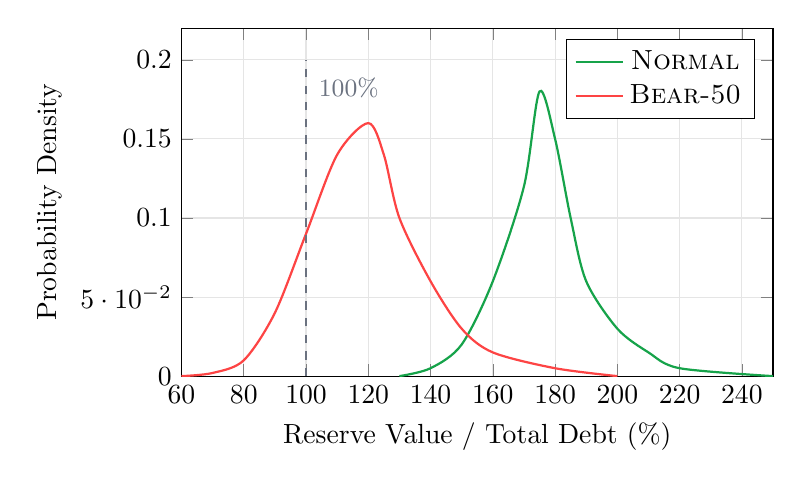
\begin{tikzpicture}
\begin{axis}[
  width=0.75\textwidth,
  height=6cm,
  xlabel={Reserve Value / Total Debt (\%)},
  ylabel={Probability Density},
  xmin=60, xmax=250,
  ymin=0,
  grid=major,
  grid style={gray!20},
  legend pos=north east,
]
% Normal
\addplot[thick, color=codegreen, smooth] coordinates {
  (130,0) (140,0.005) (150,0.02) (160,0.06) (170,0.12)
  (175,0.18) (180,0.15) (185,0.10) (190,0.06) (200,0.03)
  (210,0.015) (220,0.005) (250,0)
};
\addlegendentry{\textsc{Normal}}

% Bear-50
\addplot[thick, color=parsred, smooth] coordinates {
  (60,0) (70,0.002) (80,0.01) (90,0.04) (100,0.09)
  (110,0.14) (120,0.16) (125,0.14) (130,0.10) (140,0.06)
  (150,0.03) (160,0.015) (180,0.005) (200,0)
};
\addlegendentry{\textsc{Bear-50}}

% 100% line
\addplot[thin, dashed, color=codegray] coordinates {(100,0) (100,0.20)};
\node[anchor=south west, font=\small, color=codegray] at (axis cs:101,0.17) {100\%};
\end{axis}
\end{tikzpicture}
\caption{Distribution of aggregate collateralization ratio at epoch end. Under \textsc{Normal}, the reserve is overcollateralized in all runs. Under \textsc{Bear-50}, approximately $8\%$ of runs see the aggregate ratio briefly dip below $100\%$.}
\label{fig:reserve_dist}
\end{figure}

\section{Gas Cost Analysis}
\label{app:gas}

On-chain operations have the following estimated gas costs (EVM execution layer):

\begin{table}[H]
\centering
\caption{Estimated gas costs for reserve operations.}
\label{tab:gas}
\begin{tabular}{@{}lcc@{}}
\toprule
\textbf{Operation} & \textbf{Gas (est.)} & \textbf{Cost at 20 gwei} \\
\midrule
Open position                  & 280{,}000 & \$0.48 \\
Deposit collateral             & 120{,}000 & \$0.21 \\
Withdraw collateral            & 150{,}000 & \$0.26 \\
Mint \ashares                  & 200{,}000 & \$0.34 \\
Redeem \ashares                & 220{,}000 & \$0.38 \\
PID controller update          & 95{,}000  & \$0.16 \\
Trigger liquidation            & 180{,}000 & \$0.31 \\
Dutch auction bid              & 250{,}000 & \$0.43 \\
Oracle report (DON)            & 85{,}000  & \$0.15 \\
\bottomrule
\end{tabular}
\end{table}

The PID controller update is called once per $100$ blocks by a designated relayer.
The cost is subsidized from protocol fee revenue.

\section{Formal Invariants}
\label{app:invariants}

The following invariants must hold at all times and are candidates for formal verification:

\begin{invariant}[Accounting]
Total \ashares supply equals total debt across all positions plus protocol-held \ashares:
\begin{equation}
  \text{Supply}_{\text{ASHA-R}} = \sum_{i} d_i + B_{\text{protocol}}
\end{equation}
\end{invariant}

\begin{invariant}[Collateral Conservation]
Total collateral in the vault equals the sum of all position collateral:
\begin{equation}
  \forall a \in \mathcal{A}: \quad R_a = \sum_{i: a_i = a} c_i + R_a^{\text{surplus}}
\end{equation}
where $R_a^{\text{surplus}}$ is collateral acquired through liquidations.
\end{invariant}

\begin{invariant}[Fee Bounds]
\begin{equation}
  0 \leq f_{\text{mint}}(t) \leq 0.05, \quad 0 \leq f_{\text{redeem}}(t) \leq 0.05
\end{equation}
\end{invariant}

\begin{invariant}[Position Validity]
Every active position satisfies:
\begin{equation}
  c_i > 0 \implies d_i > 0 \quad \text{and} \quad d_i > 0 \implies c_i > 0
\end{equation}
\end{invariant}

\begin{invariant}[No Unbacked Minting]
\ashares can only be minted when backed by collateral deposited in the same transaction:
\begin{equation}
  \Delta \text{Supply}_{\text{ASHA-R}} > 0 \implies \exists a, \Delta c > 0: \text{Deposit}(a, \Delta c) \text{ in same tx}
\end{equation}
\end{invariant}

\end{document}
